\documentclass[xcolor=dvipsnames,12pt]{beamer}
\usecolortheme[named=RoyalPurple]{structure}
\useoutertheme{infolines}
\usetheme{CambridgeUS}
%\usetheme[height=14mm]{Rochester}
%\hypersetup{colorlinks=true,linkcolor=yellow}
\setbeamertemplate{items}[ball]
\setbeamertemplate{blocks}[rounded][shadow=true]
\setbeamertemplate{navigation symbols}{}
\usepackage{color}
%\usefonttheme{structuresmallcapsserif}
%\usefonttheme{professionalfonts}
%\useoutertheme{default}
%\useoutertheme{infolines}


%\documentclass{beamer}
%\usecolortheme{structure}
\usepackage{graphicx}
%\usetheme{PaloAlto}
%\setbeamertemplate{items}[ball]
%\setbeamertemplate{blocks}[rounded][shadow=true]
%\useoutertheme{umbcfootline}
\newtheorem{assume}{\rlap{A}\hskip .1in}
%\newtheorem{result}{Result}[chapter]
\newcommand{\Var}  {\mbox{Var}}
\newcommand{\V} {\mbox{V}}
\newcommand{\E}  {\mbox{E}}
\newcommand{\PR}  {\mbox{P}}
\newcommand{\diag} {\operatorname*{diag}}
\newcommand{\tr} {\mbox{tr}}
\newcommand{\bmw}[1]{{\mbox{$#1$}}}
\newcommand{\MSE}{\mbox{MSE}}
\newcommand{\MSPE}{\mbox{MSPE}}


\def\bmh{{\hat \mathbf m}}
\def\bm{{\mathbf m}}
\def\bn{{\mathbf n}}
\def\mh{{\hat m}}
\def\bOmega{{\mathbf \Omega}}
\def\be{{\mathbf e}}
\def\bs{{\mathbf s}}
\def\by{{\mathbf y}}
\def\b1{{\mathbf 1}}
\def\bx{{\mathbf x}}
\def\bw{{\mathbf w}}
\def\bzero{{\mathbf 0}}

\def\bP{{\mathbf P}}
\def\bI{{\mathbf I}}
\def\bM{{\mathbf M}}
\def\bH{{\mathbf H}}
\def\bN{{\mathbf N}}
\def\bW{{\mathbf W}}
\def\bX{{\mathbf X}}
\def\bZ{{\mathbf Z}}
\def\bT{{\mathbf T}}
\def\bV{{\mathbf V}}
\def\bC{{\mathbf C}}
\def\bG{{\mathbf G}}
\def\bY{{\mathbf Y}}
\def\bD{{\mathbf D}}
\def\bS{{\mathbf S}}
\def\bR{{\mathbf R}}

\def\bbeta{\mbox{\boldmath $\beta$}}
\def\bepsilon{\mbox{\boldmath $\varepsilon$}}

% items enclosed in square brackets are optional; explanation below
\title[]{Part 5}
%\subtitle[ttt]{}
\author[Stat 801]{Inferences about Population Variances\\
Confidence Interval for Population Variances\\
Estimation and Tests for Comparing Two Population Variances}

\date{}

\begin{document}

\begin{frame}[plain]
  \titlepage
\end{frame}




\begin{frame}
\frametitle{INFERENCES ABOUT POPULATION VARIANCES}
\textcolor{red}{Estimation and Tests for a Single Population Variance}
\begin{itemize}
\item Recall that the sample variance $s^2 = \sum(y-\bar{y})^2/(n-1)$ is the
 \textcolor{magenta}{\textit{point estimate}} of $\sigma^2$. 
\item For tests and confidence intervals about $\sigma^2$ we use the fact that the sampling random variable
$$
  (n-1) \, S^2/\sigma^2 = \chi^2
$$
has the \textcolor{magenta}{\textit{Chi-square Distribution}  with $n-1$ degrees
of freedom or $df$}, when the sample is from a normal population.
\end{itemize}
\end{frame}

\begin{frame}
\begin{itemize}
\item The chi-square distribution is nonsymmetric.
\item Like the Student's $t$
distribution, there is a different curve for each sample size
$n$ i.e., for each value of \textcolor{magenta}{\textit{df}}. 
\item Percentiles of the chi-square distribution 
are given in Table~7.
\item Plots of the chi-square distribution for $df=5, 15,$ and $30$ are shown in Fig.~7.3
\item The distribution appear to be more skewed for smaller values of $df$ and become more symmetric as $df$ increases. 
\item Because the chi-square distribution is nonsymmetric, the percentiles for probabilities at both ends needs to be tabulated.
\end{itemize}
\end{frame}


\begin{frame}
\frametitle{Chi-square Distribution}
\begin{center}
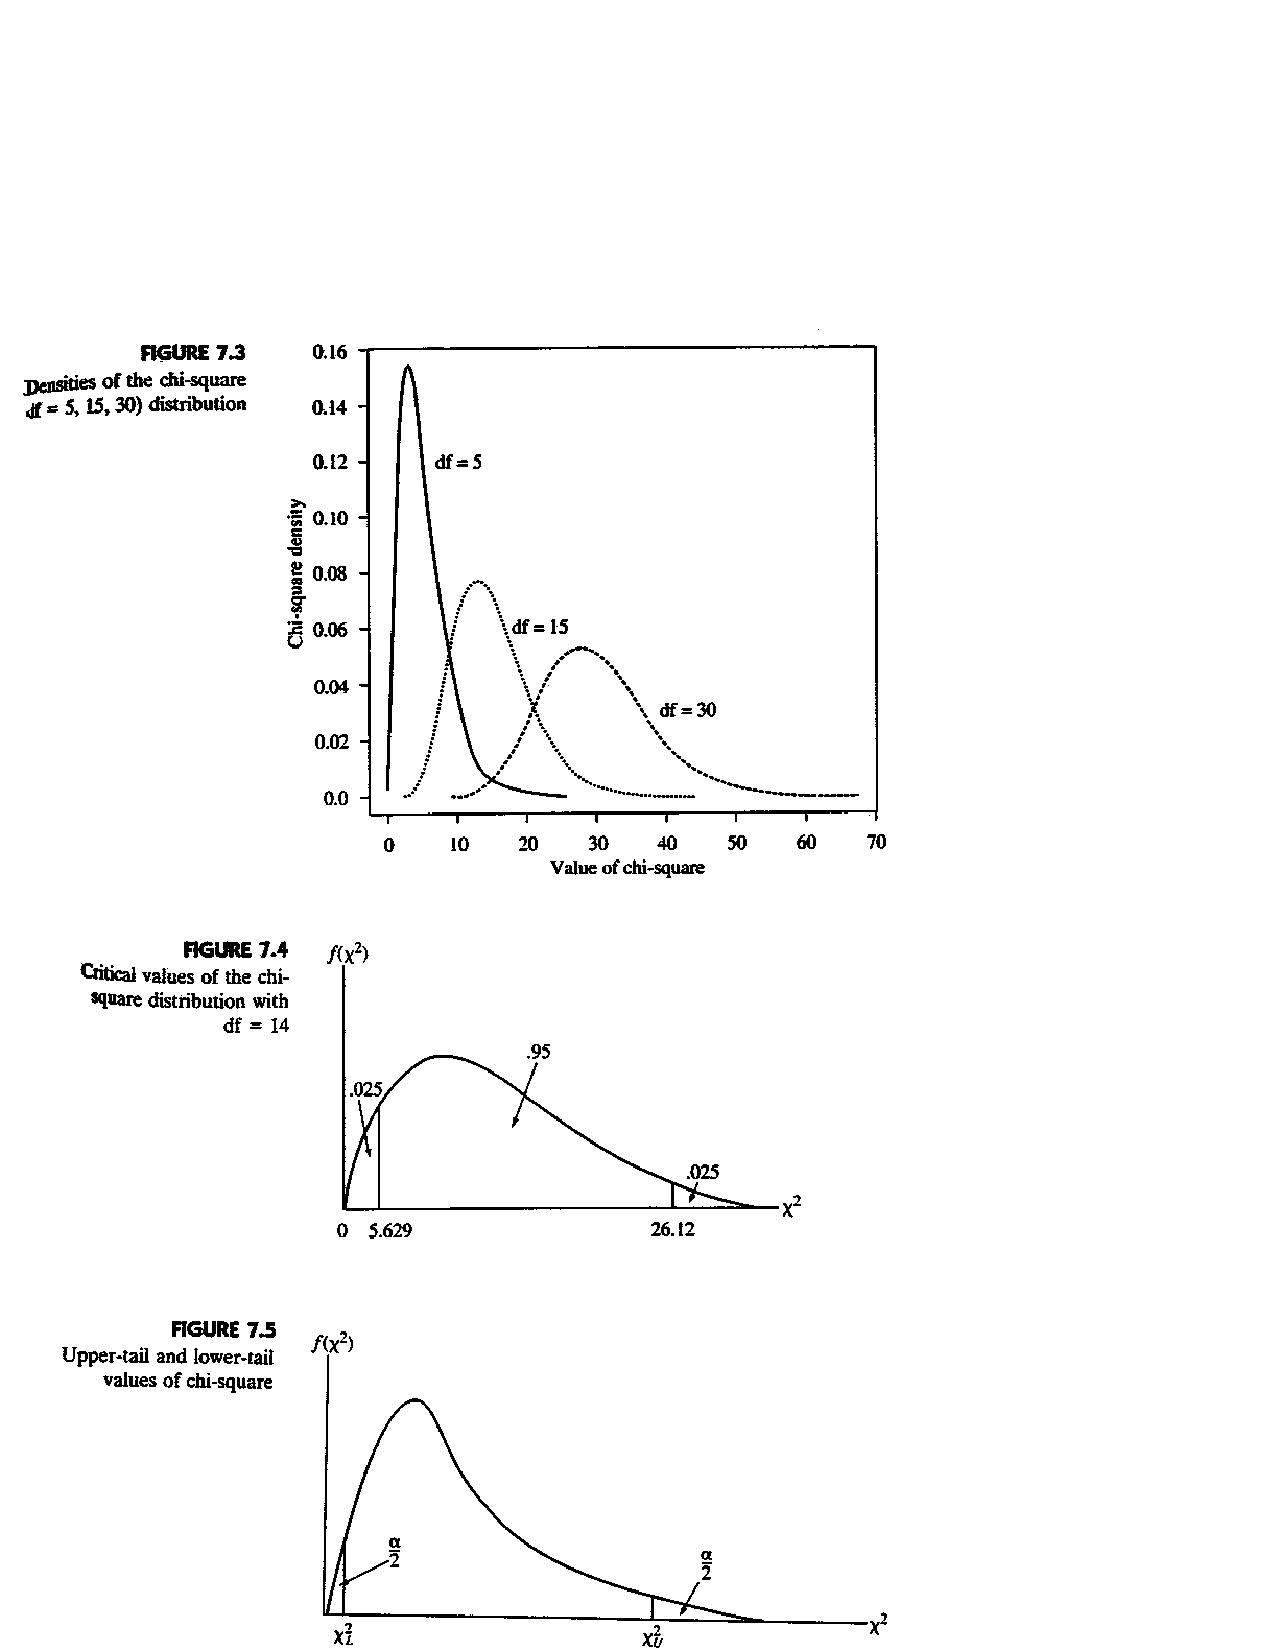
\includegraphics[trim={0cm 0cm 0cm 0cm},clip,scale=0.24]{fig73.pdf}\\[.1in]
\end{center}
\end{frame}


\begin{frame}
\frametitle{A 100(1-{\boldmath$\alpha)$}\% Confidence Interval for {\boldmath$\sigma^2$}}
 This has the form:
$$
  \frac{(n-1)s^2}{\chi_U^2} < \, \sigma^2 \, < \, \frac{(n-1)s^2}{\chi_L^2}
$$
 where \\[.01in]
 \begin{itemize}
\item Since $df = n-1$ look up $\chi_{n-1}^2$ percentiles.\\[.01in]
\item $\chi_L^2$ is the lower-tail value  with area $\alpha/2$ to the left. \\[.01in]
\item  $\chi_U^2$ is the upper-tail value with area $\alpha/2$ to the right.\\[.01in] 
\item The confidence interval for the standard deviation  $\sigma$ is found by taking square roots of both end points of above.
\end{itemize}
\end{frame}




\begin{frame}
\frametitle{Example}
Let's assume that the normal probability plot of the data  appear 
to show that the sample is from a normal distribution.\\[.1in]
From the data $n = 30$, $\bar{y} = 500.453$, $s= 3.433$ were calculated.\\[.1in]
A \textcolor{magenta}{99\% confidence interval for $\sigma^2$} is computed as follows:\\[.1in]
 Since $\alpha=.1$, \ \ $\alpha/2=.005$ and $1-\alpha/2=.995$, we compute \\[.1in]
 $\chi_L^2 =\chi_{0.995,29}^2 = 13.12 \quad \chi_U^2 = \chi_{0.005,29}^2 = 52.34$\\[.1in]
 Thus the endpoints for the required C.I. are, respectively,:\\[.1in]
\hspace*{.3in}$\frac{(n-1)s^2}{\chi_U^2} = \frac{29(3.433^2)}{52.34} = 6.53$\qquad$\frac{(n-1)s^2}{\chi_L^2} = \frac{29(3.433^2)}{13.12} = 26.05$\\[.2in]
\hspace*{.6in} Thus $(6.53,\ 26.05 )$ is a $99\%$ C.I. for $\sigma^2$
\end{frame}


\begin{frame}
Taking square roots of both endpoints of the interval for $\sigma^2$:\\[.1in]
\hspace*{.6in} we get  $(2.56,\ 5.10 )$ as a $99\%$ C.I. for $\sigma$.\\[.1in]
 Thus we are  $99\%$ confident that the standard deviation of the
weights of coffee containers lies in the interval  $(2.56,\ 5.10 )$.\\[.1in]
The filling machine was designed to be so that $\sigma = 4$ grams,
and since this value falls in the above interval, the
machine satisfies the design specification for standard deviation.\\[.1in]
 A separate confidence interval for $\mu$ is computed for
checking whether  the design specification for the mean is
satisfied. 
\end{frame}


\begin{frame}
\frametitle{Tests of Hypotheses about $\sigma^2$}
\textcolor{magenta}{Test:}
\begin{enumerate}
\item $H_0: \sigma^2 \leq \sigma_0^2$ vs. $H_a:$  $\sigma^2 > \sigma_0^2$
\item $H_0: \sigma^2 \geq \sigma_0^2$ vs. $\sigma^2 < \sigma_0^2$
\item $H_0: \sigma^2 =\sigma_0^2$ vs.  $\sigma^2 \neq \sigma_0^2$
\end{enumerate}
{\textcolor{magenta}{Test Statistic:}} \ \ $\chi^2 = \frac{(n-1)s^2}{\sigma_0^2}$\\
{\textcolor{magenta}{Rejection Region:}}  for specified $\alpha$ and $df= n-1$,\\
\begin{enumerate}
\item Reject $H_0$ if $\chi^2 > \chi_U^2$, where $\chi_U^2\equiv\chi_{\alpha,\,n-1}^2$
\item Reject $H_0$ if $\chi^2 < \chi_L^2$, where $\chi_L^2\equiv\chi_{1-\alpha,\,n-1}^2$
\item Reject $H_0$ if $\chi^2 > \chi_U^2$, where $\chi_U^2\equiv\chi_{\alpha/2,\,n-1}^2,$
 or if $\chi^2 < \chi_L^2$, where $\chi_L^2\equiv\chi_{1-\alpha/2,\,n-1}^2$
\end{enumerate}
\end{frame}

%
%
\begin{frame}
Handout - Example 7.2
\end{frame}

\begin{frame}
\frametitle{Notes about Example}
\begin{itemize}
\item The above inferences are based on the assumption of sampling from a
normal population.  
\item They are more sensitive to departures from
normality than the inferences about population mean.  
\item We don't have a CLT-type theorem which applies to $S^2$ like we have
in case of $\bar{Y}$.
\item Always plotting sample data as a preliminary procedure - using 
boxplot or normal probability  plot to look for skewness, or
outliers, is  recommended.
\end{itemize}
\end{frame}

%
%
\begin{frame}
\frametitle{Estimation and Tests for Comparing Two
Population Variances}
\begin{itemize}
\item We will consider the case of independent samples from two
populations having variances $\sigma_1^2$ and $\sigma_2^2$.
\item The main application is testing  $\sigma_1^2 = \sigma_2^2$.
\item Theory says that when the two populations are Normal, and sample
sizes are $n_1$ and $n_2$ then the random variable
$$
  F = \frac{S_1^2/\sigma_1^2}{S_2^2/\sigma_2^2} \qquad 
$$
has the $F$ distribution with degrees of freedom $df_1 = n_1-1$ and $df_2 = n_2 - 1$. 
\end{itemize}
\end{frame}


\begin{frame}
\frametitle{Estimation and Tests for Comparing Two
Population Variances - cont.}
\begin{itemize}
\item $df_1$ is the degrees of freedom associated with $S_1^2$. 
\item $df_2$ is the degrees of freedom associated with $S_2^2$. 
\item The $F$ distribution is a two parameter family indexed by
$df_1$ and $df_2$.  
\item Some use the terms \textcolor{magenta}{Numerator} and  \textcolor{magenta}{Denominator} degrees of freedom for $df_1$ and $df_2$.
\item The F-statistic is calculated as 
$$
  F_c = \frac{s_1^2/\sigma_1^2}{s_2^2/\sigma_2^2} 
$$
\item The F table gives percentiles of the F-distribution only for upper tail areas.
\end{itemize}
\end{frame}


\begin{frame}
\frametitle{Estimation and Tests for Comparing Two
Population Variances - cont.}
\begin{itemize}
\item The lower tail values, when needed can be obtained by the
relationship
$$ F_{1-\alpha,df_1,df_2}=\frac{1}{F_{\alpha,df_1^*,df_2^*}}$$
where $df_1^*=df_2$ and $df_2^*=df_1$. 
\item That is, to calculate a left tail probability, look-up the corresponding right tail probability  after switching the numerator and denominator degrees of freedom.
\item For example $F_{.95,3,10}$ is calculated using the above relationship as $1/F_{.05,10,3}=1/8.79=0.11$
\item And $F_{.95,10,3}$ is calculated using the above relationship as $1/F_{.05,3,10}=1/3.71=0.27$
\end{itemize}
\end{frame}


\begin{frame}
\frametitle{Tests comparing two variances}
{\textcolor{magenta}{Test:}} \\[.2in]
\hspace*{.6in}1. $H_0: \sigma_1^2 \leq \sigma_2^2$ \ vs.\ $H_a:\sigma_1^2 > \sigma_2^2$\\[.1in]
\hspace*{.6in}2. $H_0:\sigma_1^2 = \sigma_2^2$ \ vs.\ $H_a: \sigma_1^2 \neq \sigma_2^2$ \\[.2in]
{\textcolor{magenta}{Test Statistic:}} 
$$
  F = \frac{s_1^2}{s_2^2} 
$$ 
{\textcolor{magenta}{Rejection Region:}}  For given $\alpha$, $df_1 = n_1-1$, and $df_2 = n_2 - 1$.\\[.1in]
\hspace*{.6in}1. Reject $H_0$ if $F \geq F_{\alpha,df_1,df_2}$\\[.2in]
\hspace*{.6in}2. Reject $H_0$ if $F \leq F_{1-\alpha/2,df_1,df_2}$
or $F\geq F_{\alpha/2,df_1,df_2}$\\[.1in]
\end{frame}

\begin{frame}
\frametitle{Example}
In order to test the hypothesis $H_0: \mu_1 - \mu_2 = 0$ using a two-sample $t$-statistic with pooled sample variance, we need to assume $\sigma_1^2 = \sigma_2^2$. \\[.1in]
To check whether this is a valid assumption, let us formally test\\[.1in]
 \hspace*{.5in} $ H_0:\sigma_1^2 = \sigma_2^2\ vs.\   H_a:  \sigma_1^2 \neq
\sigma_2^2$\\[.1in]
using $\alpha=.05$\\[.1in]
 The two independent samples gave sample variances:\\[.1in] 
$ s_1^2 = 0.105, \quad s_2^2 = 0.058 $ with $df_1=9$ and $df_2=9$.
\end{frame}



\begin{frame}
\frametitle{Example - cont.}
{\textcolor{magenta}{Test:}}  $H_0:\sigma_1^2 = \sigma_2^2\ vs.\   H_a:  \sigma_1^2 \neq \sigma_2^2$\\[.1in] 
{\textcolor{magenta}{Test Statistic:}}  $F_c=\frac{s_1^2}{s_2^2}=\frac{0.105}{0.058}=1.81$\\[.1in]  
{\textcolor{magenta}{Rejection Region:}} $F \leq F_{.975,9,9}$ or $F\geq F_{.025,9,9}$\\[.1in]
From Table 8, using $\alpha$ = 0.05, $df_1 = 9$, $df_2 = 9$, we have \\[.1in]
$F_{0.025,9,9} = 4.03$ and $F_{0.975,9,9} = 1/F_{0.025,9,9}= 1/4.03=0.25$\\[.1in]
Thus we reject if $F \leq 0.25$ or  $F\geq 4.03$. \\[.2in]
Since $F_c=1.81 $ does not fall in the rejection region, we fail to reject $ H_0:
\sigma_1^2 = \sigma_2^2$.\\[.1in] 
{\textcolor{magenta}{Conclusion:}} The assumption of equal
variances for the two populations appears reasonable.
\end{frame}

%
%
\begin{frame}
\frametitle{Test comparing several variances}
{\textcolor{red}{{Hartley's $F_{max}$} Test for Homogeneity
of Variances}}\\[.1in]
 This test requires that independent random samples of equal
samples sizes, $n$, are drawn from $t$  populations having normal distributions.\\[.1in]
{\textcolor{magenta}{Test:}}  $H_0: \sigma_1^2 = \sigma_2^2=\ldots= \sigma_t^2$ 
vs. $H_a:$ Not all $\sigma^2$'s equal\\[.1in]
{\textcolor{magenta}{Test Statistic:}} 
$F_{max} = \frac{s_{max}^2}{s_{min}^2} $  where  $s_{max}^2$=largest sample variance 
 and $s_{min}^2$=smallest sample variance\\[.1in]
{\textcolor{magenta}{Rejection Region:}} For given $\alpha$,
 reject $H_0$ if $F_{max}$ exceeds the tabulated
 percentile from Table 12, for $\alpha$ .\\[.1in]
Note: Use  $t$, $df_2 = n -1$ and $a=\alpha$ to read Table 12
\end{frame}




\begin{frame}
\frametitle{Test comparing several variances cont.}
\begin{itemize}
\item  When {\textcolor{magenta}{sample sizes are not all equal}} an approximate test is
obtained if $n$ is replaced with $n_{max}$, where  $n_{max}$ is
largest sample size, in the above procedure.
\item Hartley's test is quite sensitive to violation of the normality
assumption. 
\item Thus other procedures that do not require the
normality assumption, such as Levene's test has been proposed.
\item  Levene's test is too cumbersome to
calculate by hand; so software may have to be used.  
\item Levine's  test
procedure is less powerful than Hartley's test when populations have
normal distributions.
\end{itemize}
\end{frame}
\end{document}

\newpage
%%%inserting a pic  here
\epsfig{figure=graphs/ex7_8.eps,width=5in,height=6in,angle=0,silent=1}
%

\end{document}
